\documentclass[a4paper,12pt]{article}

% ======== Packages ========
\usepackage[top=1in,bottom=1in,left=1in,right=1in]{geometry}
\usepackage{amsmath,amssymb}
\usepackage{fontspec}
\usepackage{fancyhdr}
\usepackage{booktabs}
\usepackage{listings}
\usepackage{graphicx}
\usepackage{times}
\usepackage{hyperref}
\usepackage{array}
\usepackage{xcolor}
\usepackage{float}

% ======== Fonts ========
\setmainfont{Times New Roman}
\setsansfont{Arial}
\setmonofont{Courier New}

% ======== Variables ========
\newcommand{\PaperTitle}{A Conservative and Positivity-Preserving Baseline Scheme for Shallow-Water Flow with Suspended Sediment Deposition}
\newcommand{\PaperAuthor}{Isaac Boateng Numoah}
\newcommand{\PaperDate}{June 28, 2026}

% ======== Page Header ========
\fancyhf{}
\fancyhead[R]{\sffamily \thepage}
\cfoot{}
\pagestyle{fancy}
\setlength{\headheight}{14.5pt}

% ======== Three-line Table ========
\newcommand{\threelinetable}[4]{%
  \begin{table}[htbp]
    \centering
    \caption{#1}
    \begin{tabular}{#2}
      \toprule
      #3 \\
      \midrule
      #4 \\
      \bottomrule
    \end{tabular}
  \end{table}%
}

% ======== Code Block ========
\lstset{
  frame=topbottom,
  framerule=0.55pt,
  framesep=0pt,
  basicstyle=\ttfamily\small,
  backgroundcolor=\color[gray]{0.97},
  numbers=none,
  showstringspaces=false,
  breaklines=true,
}

% ======== Document ========
\begin{document}

% ---- Title Page ----
\thispagestyle{empty}
\vspace*{4em}
\begin{center}
  \LARGE \PaperTitle
\end{center}
\vspace{2em}
\begin{center}
  \large \PaperAuthor
\end{center}
\begin{center}
  \large Old Dominion University
\end{center}
\vspace{8em}
\begin{center}
  \PaperDate
\end{center}
\vspace{3em}
\begin{abstract}
This paper studies a periodic, flat-bed, first-order finite-volume baseline for shallow-water flow coupled to suspended sediment advection and exact deposition into a separate storage variable. The scheme uses a Rusanov hydrodynamic flux, shared interface velocities computed after hydrodynamics, and a local exact deposition update. Under strict wetness and stated CFL restrictions, the baseline theorem proves exact discrete water-mass conservation, exact suspended-plus-stored sediment-volume conservation, a one-step positive-depth bound, nonnegative suspended sediment, and nonnegative concentration. Synthetic theorem-component diagnostics verify that the implementation follows these proved quantities to floating-point tolerance. The scope is restricted: there is no real-river validation, no novelty claim, no nonflat bathymetry, no open boundary, no diffusion, no wetting/drying, and no moving-bed hydrodynamic feedback.
\end{abstract}
\newpage

% ---- Contents Page ----
\pagestyle{empty}
\tableofcontents
\newpage

% ---- Main Content ----
\pagestyle{fancy}
\section{Introduction}

River-mouth morphodynamics involve coupled water motion, suspended sediment transport, deposition, and bed change. A full field-scale model must handle nonuniform beds, open boundaries, tides, wetting and drying, erosion, turbulence closures, and calibration data. This paper deliberately does not attempt that full problem. Instead, it isolates a restricted numerical baseline for which several discrete properties can be stated and proved without relying on observational data or physical validation.

The long-term motivation is an idealized two-dimensional river-mouth setting in which a channel discharges into a receiving basin. At this stage, however, the mathematical result is only for a periodic rectangular domain with a flat fixed hydrodynamic bed. Suspended sediment is represented by the conservative variable
\[
  s = h c,
\]
where \(h\) is water depth and \(c\) is a dimensionless volumetric concentration. Deposition removes suspended sediment locally and stores the same volume in a separate variable \(\beta\). The storage variable is only a sediment bookkeeping variable in the theorem; it is not used as a hydrodynamic bed elevation.

The contribution of this paper is therefore modest and specific. We define a first-order finite-volume scheme using a Rusanov shallow-water update, a first-order upwind sediment advection update, and an exact deposition step. Under periodic boundaries, strict wetness, and explicit CFL restrictions, we prove one-step water-depth positivity, nonnegative suspended sediment and concentration, exact water-mass conservation, and exact conservation of total suspended-plus-stored sediment volume in exact arithmetic.

The paper does not claim novelty, convergence of the full morphodynamic model, well-balancedness, energy stability, or validation for any real river. Existing work already contains important results on positivity-preserving and well-balanced shallow-water schemes, scalar transport, and Exner-type sediment mass balance \cite{audusse2004,kurganov2007,paola2005,karjoun2020}. The present baseline is best viewed as a transparent proof and implementation target from which later extensions can be assessed.

\pagebreak[100]
\section{Assumptions and Scope}

The theorem uses a fixed rectangular Cartesian grid with periodic indexing in both coordinate directions. The hydrodynamic bed is flat and fixed. No source term from bathymetry is present, and no well-balanced claim is made.

The water depth is assumed strictly positive at the beginning of the step:
\[
  m^n = \min_{i,j} h_{i,j}^n > 0.
\]
The gravitational constant satisfies \(g>0\), and the mesh and time-step parameters satisfy
\[
  \Delta x>0,\qquad \Delta y>0,\qquad \Delta t\ge 0 .
\]
The suspended sediment satisfies \(s_{i,j}^n\ge 0\), the settling velocity satisfies \(w_s\ge 0\), and the bed porosity parameter satisfies \(0\le \lambda_p<1\).

The model is dilute: sediment does not alter water density, pressure, or the shallow-water wave speeds. The suspended sediment is transported by the post-hydrodynamic velocity field and then deposited exactly over one time step. The diffusivity is set to zero in the theorem:
\[
  D_s = 0.
\]

The following features are excluded from the theorem and from the numerical diagnostics reported here:
\[
\begin{gathered}
\text{nonflat bathymetry, well-balancedness, diffusion, open or closed boundaries,}\\
\text{moving-bed hydrodynamic feedback, wetting/drying, tides, erosion, resuspension,}\\
\text{higher-order reconstruction, and physical validation.}
\end{gathered}
\]
These restrictions are not incidental. They are what allow the first proof to be stated without hidden boundary constructions or unproved coupling assumptions.

\pagebreak[100]
\section{Notation}

Let \(K_{i,j}\) denote the cell with indices
\[
  i=0,\ldots,N_x-1,\qquad j=0,\ldots,N_y-1,
\]
with periodic interpretation of all indices. The cell area is \(\Delta x\Delta y\). The shallow-water conservative state is
\[
  U_{i,j}^n =
  \begin{pmatrix}
  h_{i,j}^n\\ q_{x,i,j}^n\\ q_{y,i,j}^n
  \end{pmatrix},
  \qquad
  q_{x,i,j}^n=h_{i,j}^n u_{i,j}^n,\qquad
  q_{y,i,j}^n=h_{i,j}^n v_{i,j}^n .
\]
The suspended-sediment conservative variable is
\[
  s_{i,j}^n = h_{i,j}^n c_{i,j}^n,
\]
where \(c\) is dimensionless concentration. The deposited-sediment storage variable is \(\beta_{i,j}^n\), initialized by \(\beta_{i,j}^0=0\). It is separate from the flat hydrodynamic bed.

\begin{table}[H]
\centering
\caption{Main symbols}
\begin{tabular}{ll}
\toprule
Symbol & Meaning \\
\midrule
\(h\) & water depth \\
\(q_x,q_y\) & horizontal momenta \\
\(u,v\) & depth-averaged velocities \\
\(c\) & dimensionless suspended concentration \\
\(s=hc\) & suspended sediment volume per unit horizontal area \\
\(\beta\) & deposited-sediment storage, not hydrodynamic bed elevation \\
\(w_s\) & settling velocity \\
\(\lambda_p\) & porosity parameter \\
\(g\) & gravitational acceleration \\
\(\Delta x,\Delta y,\Delta t\) & grid spacings and time step \\
\bottomrule
\end{tabular}
\end{table}

\pagebreak[100]
\section{Baseline Scheme and Theorem}

\subsection{Hydrodynamic Update}

For the flat-bed homogeneous shallow-water equations, define
\[
F(U)=
\begin{pmatrix}
q_x\\ q_x^2/h+\frac12gh^2\\ q_xq_y/h
\end{pmatrix},
\qquad
G(U)=
\begin{pmatrix}
q_y\\ q_xq_y/h\\ q_y^2/h+\frac12gh^2
\end{pmatrix}.
\]
The Rusanov wave-speed bounds are
\[
a_{i+1/2,j}^n=
\max\left(|u_{i,j}^n|+\sqrt{g h_{i,j}^n},
|u_{i+1,j}^n|+\sqrt{g h_{i+1,j}^n}\right),
\]
\[
b_{i,j+1/2}^n=
\max\left(|v_{i,j}^n|+\sqrt{g h_{i,j}^n},
|v_{i,j+1}^n|+\sqrt{g h_{i,j+1}^n}\right).
\]
The numerical fluxes are
\[
\widehat F_{i+1/2,j}^n =
\frac12\left(F(U_{i,j}^n)+F(U_{i+1,j}^n)\right)
-\frac12 a_{i+1/2,j}^n\left(U_{i+1,j}^n-U_{i,j}^n\right),
\]
\[
\widehat G_{i,j+1/2}^n =
\frac12\left(G(U_{i,j}^n)+G(U_{i,j+1}^n)\right)
-\frac12 b_{i,j+1/2}^n\left(U_{i,j+1}^n-U_{i,j}^n\right).
\]
The hydrodynamic update is
\[
U_{i,j}^{n+1}
=U_{i,j}^{n}
-\frac{\Delta t}{\Delta x}
\left(\widehat F_{i+1/2,j}^n-\widehat F_{i-1/2,j}^n\right)
-\frac{\Delta t}{\Delta y}
\left(\widehat G_{i,j+1/2}^n-\widehat G_{i,j-1/2}^n\right).
\]
Let
\[
A^n=\max_{i,j}\left(|u_{i,j}^n|+\sqrt{g h_{i,j}^n}\right),
\qquad
B^n=\max_{i,j}\left(|v_{i,j}^n|+\sqrt{g h_{i,j}^n}\right).
\]
The hydrodynamic CFL condition is
\[
\Delta t\left(\frac{A^n}{\Delta x}+\frac{B^n}{\Delta y}\right)\le \frac12 .
\]

\subsection{Sediment Advection and Deposition}

After the hydrodynamic update, define
\[
u_{i,j}^{n+1}=\frac{q_{x,i,j}^{n+1}}{h_{i,j}^{n+1}},
\qquad
v_{i,j}^{n+1}=\frac{q_{y,i,j}^{n+1}}{h_{i,j}^{n+1}}.
\]
The shared interface velocities are
\[
u_{i+1/2,j}^{n+1}=\frac12\left(u_{i,j}^{n+1}+u_{i+1,j}^{n+1}\right),
\qquad
v_{i,j+1/2}^{n+1}=\frac12\left(v_{i,j}^{n+1}+v_{i,j+1}^{n+1}\right).
\]
For \(r\in\mathbb{R}\), write \(r^+=\max(r,0)\) and \(r^-=\min(r,0)\). The upwind sediment fluxes are
\[
\widehat H^x_{i+1/2,j}
=\left(u_{i+1/2,j}^{n+1}\right)^+s_{i,j}^{n}
+\left(u_{i+1/2,j}^{n+1}\right)^-s_{i+1,j}^{n},
\]
\[
\widehat H^y_{i,j+1/2}
=\left(v_{i,j+1/2}^{n+1}\right)^+s_{i,j}^{n}
+\left(v_{i,j+1/2}^{n+1}\right)^-s_{i,j+1}^{n}.
\]
The advected suspended sediment is
\[
s_{i,j}^{*}=s_{i,j}^{n}
-\frac{\Delta t}{\Delta x}
\left(\widehat H^x_{i+1/2,j}-\widehat H^x_{i-1/2,j}\right)
-\frac{\Delta t}{\Delta y}
\left(\widehat H^y_{i,j+1/2}-\widehat H^y_{i,j-1/2}\right).
\]
Let \(\lambda_x=\Delta t/\Delta x\) and \(\lambda_y=\Delta t/\Delta y\). The local outgoing-flux sediment CFL condition is
\[
\lambda_x\left[
\left(u_{i+1/2,j}^{n+1}\right)^+
-\left(u_{i-1/2,j}^{n+1}\right)^-
\right]
+
\lambda_y\left[
\left(v_{i,j+1/2}^{n+1}\right)^+
-\left(v_{i,j-1/2}^{n+1}\right)^-
\right]\le 1
\]
for every cell.

The exact deposition step is
\[
s_{i,j}^{n+1}=s_{i,j}^{*}
\exp\left(-\frac{w_s\Delta t}{h_{i,j}^{n+1}}\right),
\]
and the storage update is
\[
(1-\lambda_p)\left(\beta_{i,j}^{n+1}-\beta_{i,j}^{n}\right)
=s_{i,j}^{*}-s_{i,j}^{n+1}.
\]
The total suspended-plus-stored sediment volume is
\[
M_{\mathrm{sed}}^n=
\sum_{i,j}\Delta x\Delta y
\left[s_{i,j}^n+(1-\lambda_p)\beta_{i,j}^n\right].
\]

\subsection{Theorem}

\textbf{Theorem.}
Assume \(g>0\), \(\Delta x>0\), \(\Delta y>0\), \(\Delta t\ge0\), periodic boundaries, flat fixed hydrodynamic bed, \(D_s=0\),
\[
m^n=\min_{i,j}h_{i,j}^n>0,\qquad s_{i,j}^n\ge0,\qquad w_s\ge0,\qquad 0\le\lambda_p<1 .
\]
If the hydrodynamic CFL condition and the local outgoing-flux sediment CFL condition hold, then one time step of the scheme satisfies:
\[
\sum_{i,j}\Delta x\Delta y\,h_{i,j}^{n+1}
=
\sum_{i,j}\Delta x\Delta y\,h_{i,j}^{n},
\]
\[
m^{n+1}\ge \frac12 m^n>0,
\]
\[
s_{i,j}^{*}\ge0,\qquad s_{i,j}^{n+1}\ge0,\qquad
c_{i,j}^{n+1}=s_{i,j}^{n+1}/h_{i,j}^{n+1}\ge0,
\]
and
\[
M_{\mathrm{sed}}^{n+1}=M_{\mathrm{sed}}^n
\]
in exact arithmetic.

\subsection{Proof}

Water mass conservation follows by summing the height component of the conservative hydrodynamic update over all cells. Periodicity makes every numerical flux appear once with a positive sign and once with a negative sign, so the total flux contribution cancels.

For the depth bound, the height component of the Rusanov flux can be written as
\[
\widehat F^{(h)}_{i+1/2,j}
=\frac12\left[
h_{i,j}^n(u_{i,j}^n+a_{i+1/2,j}^n)
+h_{i+1,j}^n(u_{i+1,j}^n-a_{i+1/2,j}^n)
\right].
\]
Because \(a_{i+1/2,j}^n\ge |u_{i+1,j}^n|\), the neighbor contribution
\(h_{i+1,j}^n(u_{i+1,j}^n-a_{i+1/2,j}^n)\) is nonpositive. Applying the analogous sign argument to \(\widehat F^{(h)}_{i-1/2,j}\) gives
\[
\widehat F^{(h)}_{i+1/2,j}-\widehat F^{(h)}_{i-1/2,j}
\le A^n h_{i,j}^n.
\]
Similarly,
\[
\widehat G^{(h)}_{i,j+1/2}-\widehat G^{(h)}_{i,j-1/2}
\le B^n h_{i,j}^n .
\]
Substitution into the height update gives
\[
h_{i,j}^{n+1}
\ge h_{i,j}^{n}
\left[1-\Delta t\left(\frac{A^n}{\Delta x}+\frac{B^n}{\Delta y}\right)\right]
\ge \frac12 h_{i,j}^{n}.
\]
Taking the minimum over all cells yields \(m^{n+1}\ge m^n/2>0\).

For sediment positivity, expand the upwind update as
\[
\begin{aligned}
s_{i,j}^{*}
={}&\alpha_{i,j}s_{i,j}^{n}
+\lambda_x\left(u_{i-1/2,j}^{n+1}\right)^+s_{i-1,j}^{n}
-\lambda_x\left(u_{i+1/2,j}^{n+1}\right)^-s_{i+1,j}^{n} \\
&+\lambda_y\left(v_{i,j-1/2}^{n+1}\right)^+s_{i,j-1}^{n}
-\lambda_y\left(v_{i,j+1/2}^{n+1}\right)^-s_{i,j+1}^{n},
\end{aligned}
\]
where
\[
\alpha_{i,j}
=1-\lambda_x\left[
\left(u_{i+1/2,j}^{n+1}\right)^+
-\left(u_{i-1/2,j}^{n+1}\right)^-
\right]
-\lambda_y\left[
\left(v_{i,j+1/2}^{n+1}\right)^+
-\left(v_{i,j-1/2}^{n+1}\right)^-
\right].
\]
The local outgoing-flux CFL gives \(\alpha_{i,j}\ge0\). All other coefficients in the displayed expression are also nonnegative, since \(r^+\ge0\) and \(-r^-\ge0\). Thus \(s_{i,j}^*\) is a nonnegative linear combination of nonnegative sediment values, and \(s_{i,j}^*\ge0\). This argument is not a convex-combination argument; no discrete divergence-free condition is assumed.

The deposition multiplier is nonnegative because \(w_s\ge0\), \(\Delta t\ge0\), and \(h_{i,j}^{n+1}>0\). Therefore \(s_{i,j}^{n+1}\ge0\). The storage identity implies, cell by cell,
\[
s_{i,j}^{n+1}+(1-\lambda_p)\beta_{i,j}^{n+1}
=
s_{i,j}^{*}+(1-\lambda_p)\beta_{i,j}^{n}.
\]
The sediment advection step is conservative by periodic flux cancellation, so summing the last identity over all cells gives \(M_{\mathrm{sed}}^{n+1}=M_{\mathrm{sed}}^n\). Finally, \(c_{i,j}^{n+1}=s_{i,j}^{n+1}/h_{i,j}^{n+1}\ge0\) because the numerator is nonnegative and the denominator is strictly positive.

\pagebreak[100]
\section{Implementation Diagnostics}

The numerical work in this paper checks the implementation of the theorem components on synthetic data only. These checks do not prove the theorem; they are regression-style diagnostics for whether the implemented finite-volume formulas satisfy the same conservation, CFL, and positivity quantities used in the proof.

The reported diagnostic run used a \(48\times40\) periodic grid on \([0,1]\times[0,1]\), a smooth positive depth field, smooth periodic velocity perturbations, nonnegative suspended sediment, and initial \(\beta=0\). The final time was \(T=0.05\). At every candidate step, the code checked both the hydrodynamic CFL condition and the local outgoing-flux sediment CFL. If either bound failed, the step size was reduced and the step was recomputed from the previous accepted state.

\begin{table}[H]
\centering
\caption{Summary of theorem-component diagnostics}
\begin{tabular}{lr}
\toprule
Quantity & Value \\
\midrule
Accepted steps & \(32\) \\
Final time & \(0.05\) \\
Maximum water-mass error & \(1.1102230246251565\times 10^{-16}\) \\
Maximum total sediment-volume error & \(0.0\) \\
Minimum depth & \(0.9207608559443589\) \\
Minimum ratio \(m^{n+1}/m^n\) & \(1.000373183439133\) \\
Minimum advected sediment \(s^*\) & \(0.030045021067309604\) \\
Minimum post-deposition sediment \(s\) & \(0.030042756519181715\) \\
Minimum concentration \(c=s/h\) & \(0.030007313661758465\) \\
Maximum hydrodynamic CFL & \(0.47500000000000003\) \\
Maximum local sediment CFL & \(0.02963343875200863\) \\
Maximum global sufficient sediment CFL & \(0.08162726734897778\) \\
Total time-step reductions & \(31\) \\
\bottomrule
\end{tabular}
\end{table}

Figure \ref{fig:mass-errors} shows that the water mass and total suspended-plus-stored sediment volume remain at roundoff-level error in the diagnostic run. Figure \ref{fig:positivity} reports the tracked lower bounds for depth, advected sediment, post-deposition sediment, and concentration. Figure \ref{fig:cfl} shows that accepted time steps stay within the two CFL restrictions.

\begin{figure}[H]
\centering
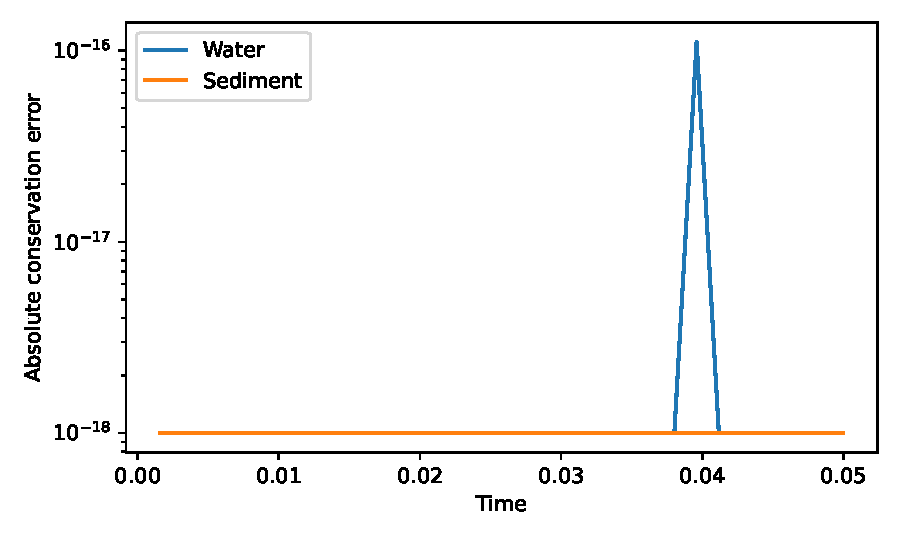
\includegraphics[width=0.82\textwidth]{figures/theorem_mass_errors.pdf}
\caption{Water-mass and sediment-volume accounting errors for the synthetic theorem diagnostic run.}
\label{fig:mass-errors}
\end{figure}

\begin{figure}[H]
\centering
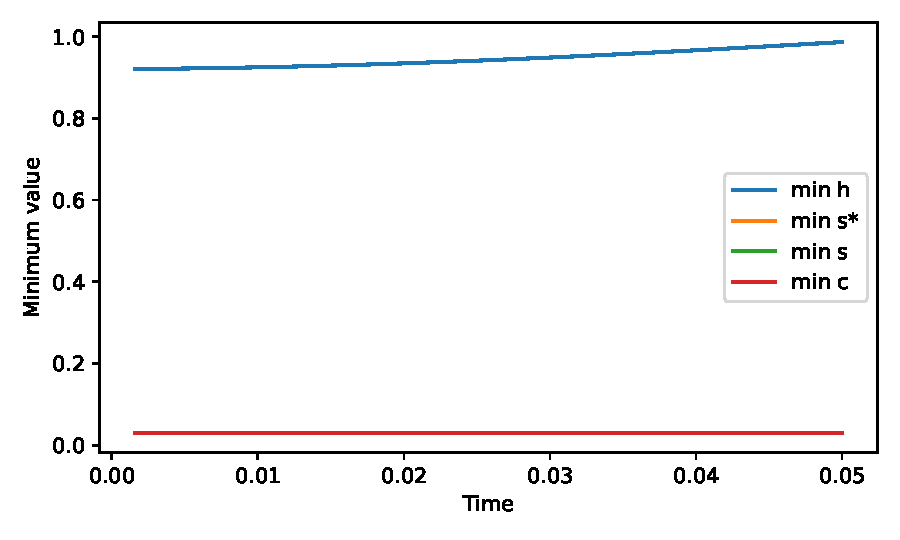
\includegraphics[width=0.82\textwidth]{figures/theorem_positivity_checks.pdf}
\caption{Tracked positivity diagnostics for depth, advected sediment, post-deposition sediment, and concentration.}
\label{fig:positivity}
\end{figure}

\begin{figure}[H]
\centering
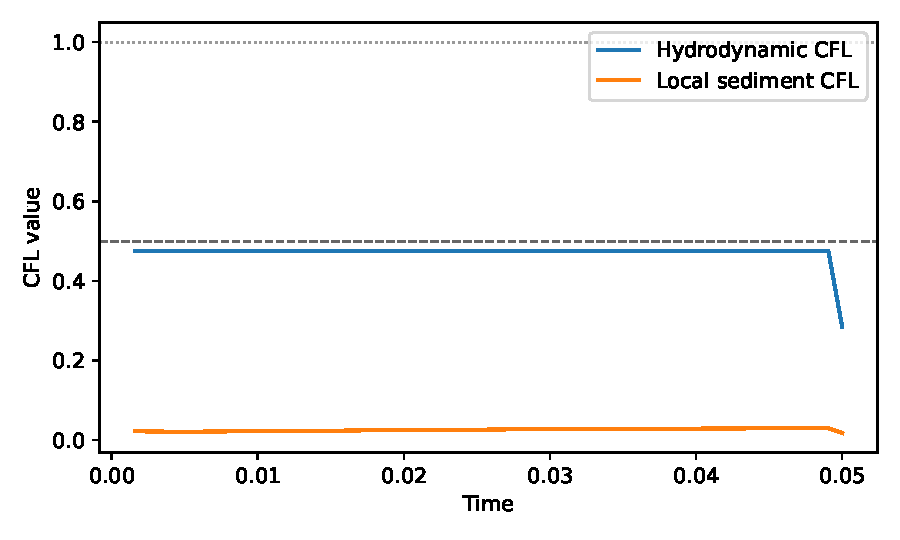
\includegraphics[width=0.82\textwidth]{figures/theorem_cfl_history.pdf}
\caption{Hydrodynamic and sediment CFL histories for accepted time steps.}
\label{fig:cfl}
\end{figure}

Additional synthetic checks were used for audit purposes: a constant periodic hydrodynamic state, a deposition-only test, a nonuniform periodic test, a near-CFL test, and a time-step retry test. The audit found that the code matches the approved finite-volume formulas and that the tests passed with tolerances of \(10^{-12}\) for mass, state, formula, positivity, and CFL diagnostics.

\section{Parameter and CFL Restrictions}

The theorem is sensitive to the explicit step-size restrictions. For the hydrodynamic part, the sufficient condition is
\[
\Delta t\left(\frac{A^n}{\Delta x}+\frac{B^n}{\Delta y}\right)\le\frac12.
\]
This bound is used only as a sufficient condition for the one-step lower bound \(m^{n+1}\ge m^n/2\); it is not asserted to be sharp.

For sediment advection, the local outgoing-flux condition is checked cell by cell. A global sufficient bound is
\[
2\Delta t\left(\frac{U_s^{n+1}}{\Delta x}+\frac{V_s^{n+1}}{\Delta y}\right)\le1,
\]
where
\[
U_s^{n+1}=\max_{i,j}|u_{i+1/2,j}^{n+1}|,
\qquad
V_s^{n+1}=\max_{i,j}|v_{i,j+1/2}^{n+1}|.
\]
The implementation uses the local condition for acceptance and records the global bound as an additional diagnostic.

The settling velocity \(w_s\) appears in the exact deposition multiplier
\[
\exp\left(-\frac{w_s\Delta t}{h_{i,j}^{n+1}}\right).
\]
For \(w_s\ge0\), this multiplier is nonnegative and no larger than one. Thus deposition cannot create negative suspended sediment in exact arithmetic. Very large \(w_s\Delta t/h\) can, however, make the suspended part extremely small in floating-point arithmetic; this is an implementation concern rather than a change in the exact discrete identity.

No full parameter sensitivity study is claimed here. Tidal forcing, open boundaries, nonflat beds, diffusion, and moving-bed feedback are later numerical extensions, not components of the theorem or the diagnostics in this paper.

\section{Evaluation and Limitations}

The main strength of the baseline is that each proved property has a clear discrete mechanism. Water mass and sediment advection are conservative because of periodic flux cancellation. Suspended-to-stored sediment transfer is exact because the same removed suspended volume is inserted into \(\beta\). Positivity of \(s^*\) follows from a nonnegative linear-combination argument under the local outgoing-flux CFL. Positivity of \(c\) follows only after the hydrodynamic step has produced a strictly positive depth.

The main weakness is the narrow scope. Periodic boundaries avoid boundary flux choices and are not a river-mouth boundary condition. The flat bed avoids source-term balance issues. The storage variable \(\beta\) does not feed back into the shallow-water update. The theorem also omits diffusion, erosion, resuspension, wetting and drying, and higher-order reconstruction.

The numerical figures should be read accordingly. They verify selected implementation diagnostics on synthetic test cases, but they do not replace the mathematical proof and do not validate the model for a physical estuary or river mouth.

\pagebreak[100]
\section{Conclusions}

This paper formulated and proved a restricted baseline theorem for a first-order periodic finite-volume scheme coupling shallow-water hydrodynamics, suspended sediment advection, exact deposition, and deposited-sediment storage. Under explicit CFL restrictions and strict wetness, the scheme conserves water mass, conserves total suspended-plus-stored sediment volume, preserves nonnegative suspended sediment and concentration, and satisfies the one-step lower bound \(m^{n+1}\ge m^n/2>0\).

The computational diagnostics are consistent with the theorem specification and with the independent code audit. The results are intentionally limited to synthetic verification of the approved baseline implementation.

Future work should treat nonflat bathymetry, well-balancedness, nonperiodic boundaries, diffusion, erosion and resuspension, moving-bed hydrodynamic feedback, wetting and drying, higher-order accuracy, and convergence studies. Each extension should be accompanied by a separate proof target or explicitly labeled as numerical evidence only.


% ---- References ----
\pagebreak[100]
\addcontentsline{toc}{section}{References}
\begin{thebibliography}{9}

\bibitem{audusse2004}
E. Audusse, F. Bouchut, M.-O. Bristeau, R. Klein, and B. Perthame.
\newblock A fast and stable well-balanced scheme with hydrostatic reconstruction for shallow water flows.
\newblock \emph{SIAM Journal on Scientific Computing}, 25(6):2050--2065, 2004.

\bibitem{kurganov2007}
A. Kurganov and G. Petrova.
\newblock A second-order well-balanced positivity preserving central-upwind scheme for the Saint-Venant system.
\newblock \emph{Communications in Mathematical Sciences}, 5(1):133--160, 2007.

\bibitem{paola2005}
C. Paola and V. R. Voller.
\newblock A generalized Exner equation for sediment mass balance.
\newblock \emph{Journal of Geophysical Research: Earth Surface}, 110:F04014, 2005.

\bibitem{karjoun2020}
H. Karjoun, A. Beljadid, and P. G. LeFloch.
\newblock A well-balanced and positivity-preserving finite volume scheme for surface water flow and transport.
\newblock arXiv:2012.13702, 2020.

\end{thebibliography}


% ---- Appendices ----
\pagebreak[100]
\appendix
\section{Reproducibility Notes}
The implementation used for the diagnostics follows the finite-volume formulas in Section 4. The essential accepted-step logic is:
\[
\begin{array}{l}
\text{propose } \Delta t,\\
\text{check the hydrodynamic CFL and recompute if it fails,}\\
\text{apply the Rusanov shallow-water update,}\\
\text{compute post-hydrodynamic interface velocities,}\\
\text{check the local outgoing-flux sediment CFL and recompute if it fails,}\\
\text{apply upwind sediment advection, exact deposition, and the }\beta\text{ update,}\\
\text{record mass, sediment-volume, positivity, and CFL diagnostics.}
\end{array}
\]
Rejected trial steps do not overwrite the previously accepted state. The synthetic diagnostics use no downloaded data and no field calibration.

The figures in Section 5 were generated from the recorded theorem diagnostics. The audit used tolerance \(10^{-12}\) for mass conservation, sediment-volume accounting, constant state preservation, positivity lower bounds, deposition formula checks, and CFL limits. These tolerances describe floating-point implementation checks; they are not assumptions in the exact-arithmetic theorem.


\end{document}
